
\chapter{FDTD} \label{ch:fdtd}


\section{Overview}

FDTD expresses Maxwell's equations as a set of discretized time-domain equations\cite{Yee}. These equations describe each electric field component in terms if its orthogonal, coupled magnetic fields, and each magnetic field component as a function of its coupled electric fields.


\section{Wave equation}

In a time-domain simulation, the wave equation for  $ E_z $ is of the form:

\begin{equation} \label{eq:waveequation} 
\frac{\partial E_z}{\partial t} = K * (\frac{\partial H_x}{\partial y} + \frac{\partial H_y}{\partial x})
\end{equation}

Equation \ref{eq:waveequation} states that the temporal derivative (change in amplitude) of $E_z$ is a function of the $Y$-axis spatial derivative of the $H_x$ field and the $X$-axis spatial derivative of the $H_y$ field.


In order to apply this equation to a computational domain, FDTD defines a discretization strategy. The simulation domain is divided into cells, and each frame is updated using a fixed time step derived from parameters such as source wavelength and simulation dimensionality.


\section{Yee Cell}

Yee \cite{Yee} defines a computational unit known as a "cell." The cell describes how each field component within a domain is related to it's coupled fields. For instance, each $E_Z$ field component depends on adjacent $H_y$ and $H_x$ components. The cell format used in such a simulation is of the form shown in \autoref{fig:yeecell}.

\begin{figure}[H]
	\centering
	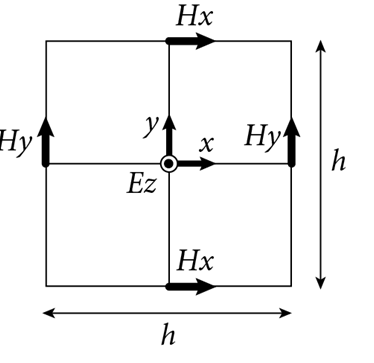
\includegraphics{yee-cell-ez.png}
	\caption{2D $TM_Z$ Yee Cell}
	\label{fig:yeecell}
\end{figure}

More formally, we may expand the $E_Z$ wave equation, arriving at:

\begin{equation} \label{eq:ezupdate}
{E_z}_{i,j}^{t} = C_a * {E_z}_{i,j}^{t-1} 
+ C_b * ({H_x}_{i,j+\frac{1}{2}}^{t-\frac{1}{2}} - {H_x}_{i,j-\frac{1}{2}}^{t-\frac{1}{2}})
+ C_b * ({H_y}_{i+\frac{1}{2},j}^{t-\frac{1}{2}} - {H_xy}_{i-\frac{1}{2},j}^{t-\frac{1}{2}})
\end{equation}

Similarly, the equations for the coupled fields $H_x$ and $H_y$ may be expressed as:
\begin{equation} \label{eq:hxupdate}
{H_x}_{i,j}^t = D_a * {H_x}_{i,j}^{t-1} + D_b * (
{E_z}_{i,j+\frac{1}{2}}^{t-\frac{1}{2}} 
-
{E_z}_{i,j-\frac{1}{2}}^{t-\frac{1}{2}}
)  
\end{equation}

\begin{equation} \label{eq:hyupdate}
{H_y}_{i,j}^t = D_a * {H_y}_{i,j}^{t-1} + D_b * (
{E_z}_{i+\frac{1}{2},j}^{t-\frac{1}{2}} 
-
{E_z}_{i-\frac{1}{2},j}^{t-\frac{1}{2}}
)  
\end{equation}

\iffalse
From Nathan:

You need to expand this a fair amount more.  You need to at minimum define all of the terms in these equations.  A paragraph or two on how a full domain is discritized, and how a simulation steps in 1/2 detla T steps is important.  

This will be important in the discussion between CPU and GPU architectures as you want to list how with FDTD you calcuate an entire time step, or 'frame' over the entire phyisical domain before moving on to the next frame.  You can state here how the updates of frames are independent of other calculations done during that same frame
\fi

\begin{table}[h!]
	\centering
	\caption{FDTD Equation Terms}
	\label{tab:modelColorComponentUsage}
	\begin{tabular}{l | c | l}
		Symbol	& Definition & Description \\
		\hline				\\										 	 
		$i$ 	& &	Field element location along the domain $X$ axis  \\
		$j$   	& &	Field element location along the domain $Y$ axis  \\
		$t$   	& &	Time step ($t_E = t_H \frac{+}{-}\frac{1}{2}$) \\
		$E_Z$ 	& &Electric field amplitude in $Z$ \\
		$H_X$ 	& &Magnetic field amplitude in $X$ \\
		$H_Y$	& &Magnetic field amplitude in $Y$ \\
		$C_a$	& &Permittivity of free space	\\
		$C_b$	& $\frac{1}{\sqrt{\epsilon_0 \epsilon_R}}$ & Permittivity at the location $i,j$\\
		$D_a$	& 	& Permeability of free space \\
		$D_b$	& $\frac{1}{\sqrt{\mu_0 \mu_r}}$	& Permeability at the location $i,j$\\
	\end{tabular}
\end{table}


\subsection{FDTD in SIMD}

FDTD's leap-frog update method, whereby E fields and H fields are successively calculated, is well-suited to a GPU implementation. E field values depend on adjacent H field values, and visa-versa. Since the E-field update equation requires knowledge only of the H field state and previous E field state, each field component can be calculated independently with no opportunity for a pipeline stall or race condition. 

